% This file is isea.tex.  It contains the formatting instructions for and acts as a template for submissions to ISEA 2015.  It is based on the ICCC  formats and instructions.  It uses the files isea.sty, isea.bst and isea.bib, the first two of which also borrow from AAAI IJCAI formats and instructions.
% Modified from ICCC.tex by B. Bogart

\documentclass[letterpaper]{article}
\usepackage{isea}
\usepackage[pdftex]{graphicx}
\usepackage{times}
\usepackage{helvet}
\usepackage{courier}
\usepackage[numbers]{natbib}
\usepackage[normalem]{ulem}
\useunder{\uline}{\ul}{}
\pdfinfo{
/Title (Accelerating Real-World XDP Programs Using HW-based Hints)
/Author (Peter P. Waskiewicz Jr)}
% The file isea.sty is the style file for ISEA 2015 proceedings.
%
\title{Accelerating Real-World XDP Programs Using HW-based Hints}
\author{Peter P. Waskiewicz Jr. \\ Intel \\ Hillsboro, OR, USA \\ peter.waskiewicz.jr@intel.com
\And Neerav Parikh \\ Intel \\ Hillsboro, OR, USA \\ neerav.parikh@intel.com
\newline
\newline
}
\setcounter{secnumdepth}{0}

\begin{document} 
\maketitle
\begin{abstract}
This talk is a continuation of the initial XDP HW-based hints work presented at NetDev 2.2 in Seoul, South Korea.

It will will start with focus on showcasing new prototypes to allow an XDP program to request required HW-generated metadata hints from a NIC. The talk will show how the hints are generated by the NIC and what are the performance characteristics for various XDP applications. We also want to demonstrate how such a metadata can be helpful for applications that use AF\_XDP sockets.

The talk with then discuss planned upstreaming thoughts, and look to generate more discussion around implementation details, programming flows, etc., with the larger audience from the community.
\end{abstract}

\section{Keywords}

networking, kernel, ebpf, xdp, offloads, performance

\section{Introduction}
XDP continues to evolve and grow in its capabilities and features for a growing number of workload types.  In order to continue maximizing the efficiency and performance of XDP, focus on offloading pieces of the processing to hardware is key.  Initially shared at NetDev 2.2 in Seoul, South Korea in Nov. 2017 \cite{xdp-acceleration-2017}, the initial proposal explored a simple theoretical case of improving XDP performance using hardware-provided metadata.  This paper will continue that exploration, which will cover:
\begin{itemize}
\item How does this HW-provided metadata help real-world XDP applications?
\item What happens to performance when hardware is actually generating this metadata inline with packet data, versus through descriptors or synthesized in the driver itself?
\item What new applications should be focused on next?
\item How can BPF Type Format (BTF) be used to program which HW-provided metadata XDP applications wish an underlying driver/device to generate and present to the application?
\end{itemize}

\section{HW Offloaded Hints From Device Driver - Recap} 
In the initial work and testing done to try and improve XDP performance using HW-generated hints, the focus was mostly on the kernel and driver interfaces that would need to change.  The introduction of the {\small \texttt{data\_meta}} pointer inside the {\small \texttt{xdp\_buff}} was the start of the required groundwork.  This allowed a driver to begin placing data, either via {\small \texttt{memcpy()}} or through other ways (e.g. DMA directly if the device supported DMA to pre-packet payloads).
\newline
\newline
What the data showed is that there was promise for this work.  In Figure \ref{xdp-program-performance}, the XDP\_HINTS program, which is a modified version of the simple XDP1 sample program, would look at the packet type as reported by the driver.  It would then decide to drop the packet or not if it matched a certain packet type.  The difference here though is the XDP program itself didn't parse the packet header, rather the program consumed the metadata provided by the driver and ultimately the hardware.  This led to a large performance increase of the XDP application, where it eventually hit a hardware limit in the test setup.

\begin{figure}[h]
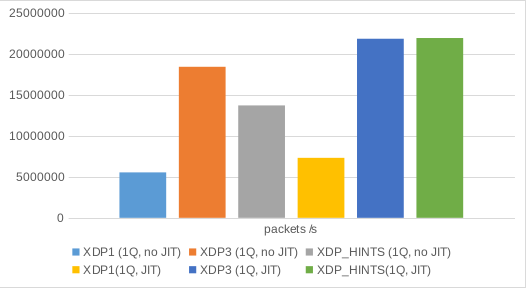
\includegraphics[width=3.31in]{xdp-programs-performance.png}
\caption{XDP With and Without HW Hints}
\label{xdp-program-performance}
\end{figure}

\section{Real-World Application: Layer 4 Load Balancer}
One of the most effective applications that XDP can support is a network load balancer.  Facebook released their Katran load balancer as open-source \cite{katran-2018} which at its core is an XDP application.  This is what they employ as their main edge load balancer, which showcases how effective XDP is by running one of the largest data centers in the world.
\newline
\newline
Using a simple version of this layer 4 (L4) load balancer, instrumentation was done to the i40e driver \cite{xdp-patches-2018} and to the simple L4 LB to consume metadata that was “generated” by the device.  In this scenario, the metadata was inserted into the {\small \texttt{data\_meta}} section of the {\small \texttt{xdp\_buff}} by the driver via {\small \texttt{memcpy()}}, as the i40e device in use does not currently have the ability to DMA metadata prior to packet data.  So consider this metadata partially synthesized.
\newline
\newline
The metadata that was synthesized and provided was a combination of packet type (as identified by the i40e hardware), and a tuple that included TCP/UDP source/destination ports, IP addresses, and the packet hash index (RSS) generated by hardware.

\subsection{Without state or connection tracking}

\begin{figure}[h]
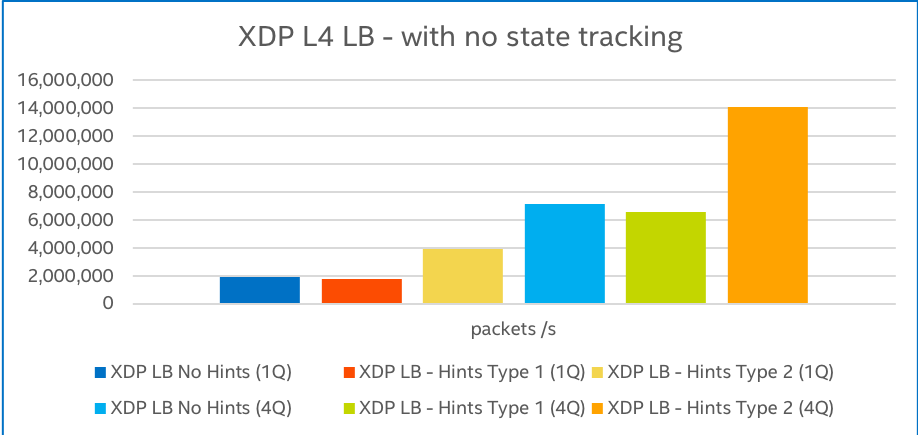
\includegraphics[width=3.31in]{l4-perf-no-tracking.png}
\caption{L4 LB with Hints, No State Tracking}
\label{l4-perf-no-tracking}
\end{figure}

In Figure \ref{l4-perf-no-tracking}, the data is showing performance of the L4 LB across various configurations.
\newline
\newline
In Type 1 Hints, the metadata being provided by the driver is the packet type (e.g. IPv4/TCP, IPv6/UDP, etc.).  These packet types are what the i40e hardware identifies off the wire, and are not yet standardized in the network stack.  However, the L4 LB is modified in this situation to match the i40e packet types.
\newline
\newline
In Type 2 Hints, the metadata being provided by the driver is metadata from Type 1, but then also includes the Source/Destination Port, Source/Destination IP Addresses, and the packet index type (RSS) generated by the hardware.
\newline
\newline
These tests are running in a stateless configuration, meaning, the XDP application is not maintaining any connection state tracking.  In other words, there are no map entries being created for new connections, and map entries being destroyed on gracefully closed connections.  This eliminates a large amount of overhead, and can be seen in the scalability of the testing a 4 queues with Type 2 hints, running at approximately 14 million packets/second.  Compare this to no driver-provided hints with 4 queues, and the test can run at roughly half the performance, or 7 million packets/second.

\subsection{With State and Connection Tracking}

\begin{figure}[h]
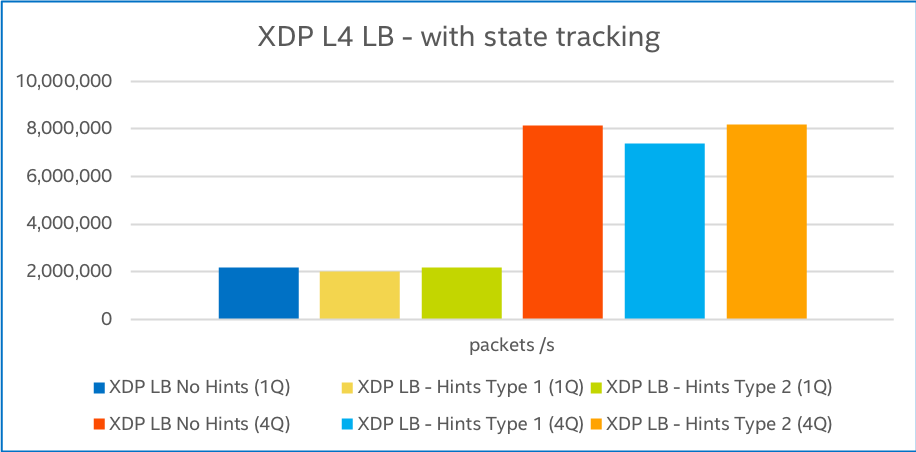
\includegraphics[width=3.31in]{l4-perf-with-tracking.png}
\caption{L4 LB with Hints, With State Tracking}
\label{l4-perf-with-tracking}
\end{figure}
In Figure \ref{l4-perf-with-tracking}, a more real-world scenario is presented for the L4 LB.  This includes the tracking of connections and state of those connections, which will require many more accesses to the eBPF maps.  The metadata presented is the same as in the tests without connection and state tracking.
\newline
\newline
Between the two main tests, each using 4 queues, Type 2 hints and no hints at all perform the same, approximately 8.1 million packets/second.  Unfortunately the large number of map hits are the majority of the execution pipeline, where the HW-generated metadata hints cannot help in this situation.  The gains seen in the data processing of the actual packet are just a fraction of the overall cost to the load balancer.  In other words, with state tracking, a L4 LB with this approach using these tests with synthesized hints will not see much benefit or performance gain.

\subsection{Projected Performance Increase}
In the stateless and stateful L4 LB tests, the method of generating the metadata inside the {\small \texttt{xdp\_buff}} struct was to {\small \texttt{memcpy()}} the data into the {\small \texttt{data\_meta}} section of the payload.  This isn’t the most ideal situation, since this can more than certainly cause cache misses, and incur additional overhead while trying to process data.
\newline
\newline
As seen in Figure <insert new figure here>, extrapolation can be done by breaking down cycle counts for the stateful L4 LB tests.  Observing the number of cycles being spent in the i40e driver to synthesize the metadata, and the subsequent {\small \texttt{memcpy()’s}} of information into the {\small \texttt{xdp\_buff}} metadata payload, cycles are available to save if the underlying hardware placed the metadata directly into the {\small \texttt{xdp\_buff}} during DMA.  With the dataset from the stateful tests, that could provide an addition 5\% throughput in the Type 2 Hints with 4 queues test.

\section{Future Application Research}
Given the current challenges of little to no gain in performance using Type 2 hints with XDP applications with stateful tracking, additional applications should be considered.  Distributed Denial of Service (DDoS) attacks are very effectively mitigated using XDP, since there is no state tracking outside of blacklist (or whitelist) ranges to drop.  The XDP application itself does not require maintenance of the DDoS blacklist maps, and only requires lookups to decide the packet action, where stateful trackers will also change and update maps.
\newline
\newline
Future testing is planned for these types of applications, where the Type 2 Hints with no state tracking is showing significant increases in performance with the L4 LB (100\% increase).

\section{BTF Integration: Expressing Requested Hints}
At NetDev 2.2, that work explored changes to LLVM and the entire toolchain to include a requested hints section in the eBPF binary.  This would be passed through the eBPF load mechanisms, and then eventually intercepted and passed to the underlying driver to program the hardware to generate the requested hints.  This was purely a proposal to get discussion going.
\newline
\newline
With the recently-added BPF Type Format (BTF) to the Linux kernel \cite{btf-patches-2018}, this tooling is now mostly in place.  This allows different metadata structures to be defined through the BTF framework.  However, this is just the top half of the solution.
\newline
\newline
What is needed to finish this tooling is intercepting the BTF structures defined for the requested metadata, and pass that into a driver to program the underlying hardware.  Preliminary work being done by Mellanox (citation needed) is showing progress in this space.  To get to a truly flexible model where an XDP application can request metadata and then use what a driver provides will require this BTF framework to evolve and mature.

\section{Conclusion}
Initial thoughts whether or not XDP could benefit from HW-generated metadata in real-world applications are proven that this is the case.  Utilizing hardware, especially as it becomes smarter and more flexible, will continue pushing XDP’s performance envelope.  In the span of a year, this has moved from a purely theoretical hope of improvement, to showing it can help in real-world applications.  The next steps needed to make this part of the XDP core is the ability to flexibly program the driver and hardware using the BTF framework.  And as hardware capabilities allow the DMA of metadata as part of the packet payloads, then more XDP applications will benefit from performance gains across the board.

\section{Acknowledgments}
We would like to acknowledge the Linux Plumbers Networking Track selection committee for inviting us to submit and present this paper.

\bibliographystyle{xdp-plumbers-2018}
\bibliography{xdp-plumb ers-2018}

\section{Author Biographies}
Peter Waskiewicz Jr (PJ) is a Senior Linux Kernel Engineer in the Networking Division of Intel's Communications Group. He has maintained and helped create the igb, ixgbe, and i40e wired Ethernet network drivers, the initial Tx multiqueue support in the Linux kernel network stack, and added Data Center Bridging support to the Linux kernel. He also worked in Intel's Open Source Technology Center on the x86 kernel tree, enabling advanced features in the Broadwell and Skylake microarchitectures. Prior to returning to Intel, PJ was a Principal Engineer at NetApp in the SolidFire division, where he was the chief Linux kernel and networking architect for the SolidFire scale-out cloud storage platform.
\newline
\newline
Neerav Parikh is a Software Architect with Intel's Connectivity Group focusing on Ethernet Networking Software. He has worked on Intel's ixgbe and i40e Linux device drivers, focusing on features related to FCoE, DCB, and QoS. Prior to joining Intel, Neerav worked as a Technical Architect enabling SAS/SATA/FC-based Storage software products.

\end{document}
